
\subsubsection{Project Description}
In a production line operated by robots, speed is of the utmost importance. 
One of the applications of our work at IIT is an automated vegetable picking and binning.
After the object is picked, it should be quickly placed in a bin across the robot's workspace.
To increase the frequency of this operation, high accelerations and velocities need to be achieved by the robot.
However, this rapid movements generate forces at the object, which may cause it to slip away or to be projected out of the robot hand.

\subsubsection{Task Overview}
The task consists of, given a grasped object and a reference trajectory to place it in the bin, find an optimal modified trajectory such that the robot does not lose the object when travelling at a high velocity.
While the final location of the object is fixed, the robot can for example turn its wrist such that it resists against acceleration and centrifugal forces  at that particular part of the trajectory.

\begin{figure}[htb!]
	\centering
	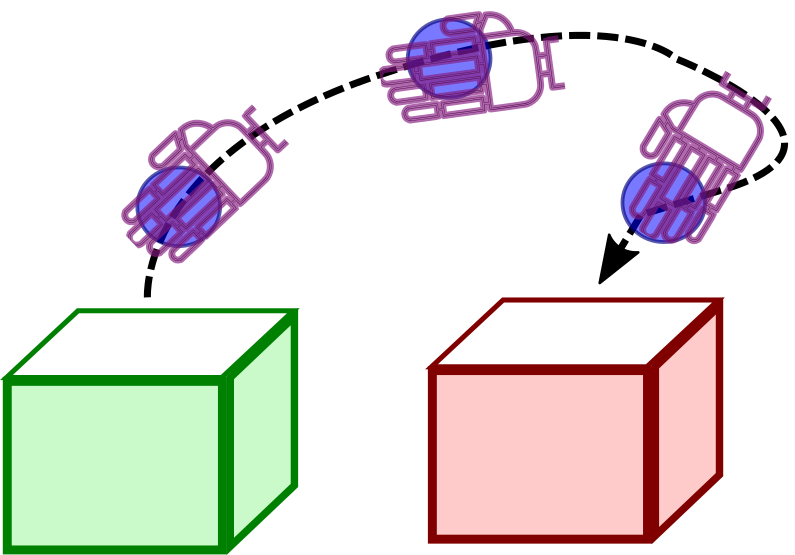
\includegraphics[width=6cm]{transport}
	\caption{Adjustment of the hand orientation to prevent slippage}
\end{figure}
\subsubsection{Timeline}
\paragraph{Months 1-2}
The student should dedicate the first two months of his project to getting familiar with the hardware and software architecture.
Tutorials and online courses in C++, Python, and ROS (Robot Operating System) programming should be followed, while also learning how to interface with the hardware.
\paragraph{Months 3-4}
During the second part of the project, the student should learn and implement rigid body dynamics algorithms to predict the forces that will be acting on the object.
He should also obtain a model of the forces that a grasp can resist and modify the end-effector orientation trajectory such that it can resist these forces.
\paragraph{Months 5-6}
In the last part of the project, the developed methods should be implemented on the robot. Performance should be thoroughly tested and a scientific article may be prepared.
\subsubsection{Required Skills}
The successful completion of this project requires that the student possesses or can easily acquire the following skills: 
%\subsection{Technical Skills}
\paragraph{Programming} A significant part of the work will be the development of algorithms and control laws to be executed by the robot. Prototyping is usually done in MATLAB and then implemented in the C++ or Python programming languages.
\paragraph{Linear Algebra} Knowledge of Linear Algebra is essential for developing robot motion control algorithms, particularly  transformations, Jacobian matrices, and matrix operations.
\paragraph{Rigid Body Dynamics} 
The student should learn rigid body dynamics and algorithms to implement them.
In particular, the student should learn forward and inverse kinematics and dynamics, Newton-Euler equations, inertial forces.
\paragraph{Grasping} 
Understanding of force and form closure, stiffness matrices, grasp matrix.

\subsubsection{Outcomes}
The student will become proficient in robot dynamics and motion control. 
Furthermore, he will have the experience of working in a \textbf{research} environment, obtaining \textbf{experimental} skills, the ability to work independently and in a group. He will also learn how to do data analysis, scientific writing, systems engineering and programming.
The results of the student project will be included in the final demonstrator to be presented to project reviewers.